\documentclass[a4paper,10pt]{article}
\usepackage[utf8]{inputenc}
\usepackage{graphicx}

%http://tex.stackexchange.com/questions/17489/change-caption-name-of-figures
\renewcommand{\figurename}{Step}

%opening
\title{Mash Cleaning}
\author{Ryan Duve}

\begin{document}

\maketitle

\begin{abstract}
\vspace{.1cm}
\fbox{\parbox{.75\textwidth}{Only workers highly familiar with the technical aspects of Hifrost are authorized to perform this procedure.
}}
\vspace{.1cm}

The mash that came from Germany has an unknown amount of air or water vapor in it.  We will clean it according the following procedure.

\end{abstract}

\section{Prep}
\begin{figure}[htbp!]
 \centering
 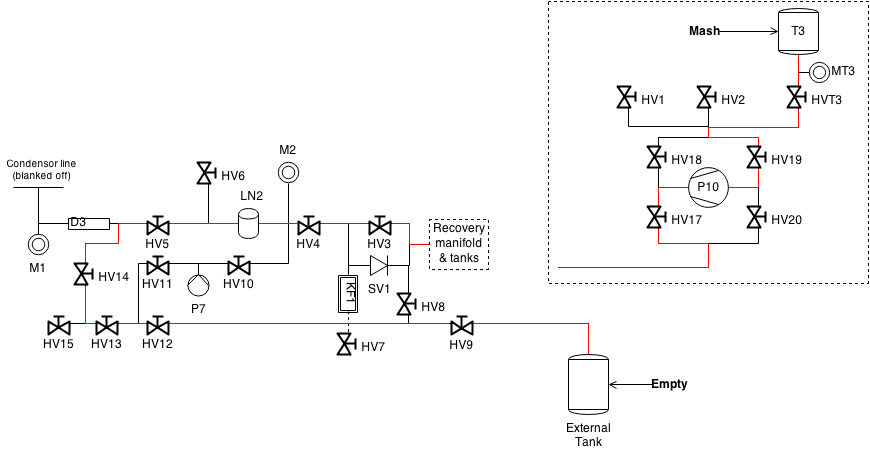
\includegraphics[width=\textwidth]{./mash-cleaning-schematic-1.png}
 % he-3-transfer-04-evac-system-with-p7.png: 0x0 pixel, 0dpi, 0.00x0.00 cm, bb=
 \caption{Hook up system as shown.  Red channels indicate the mash transport path from T1 to the external tank.}
 \label{a}
\end{figure}

\begin{itemize}
 \item Regenerate LN$_2$ trap.
 \item Evacuate T3 with P7 (for trapped air measurement).
 \item Configure the system as shown in Step \ref{a}. Purge all lines along the transport path (keeping HV1 closed!) with P7 to clean the system.
 \item Leak check the external tank and new connections (e.g., blanked condensor line).
 \item Close all valves; kill P7; fill trap with LN$_2$.
\end{itemize}

\section{Cleaning}

\begin{figure}[htbp!]
 \centering
 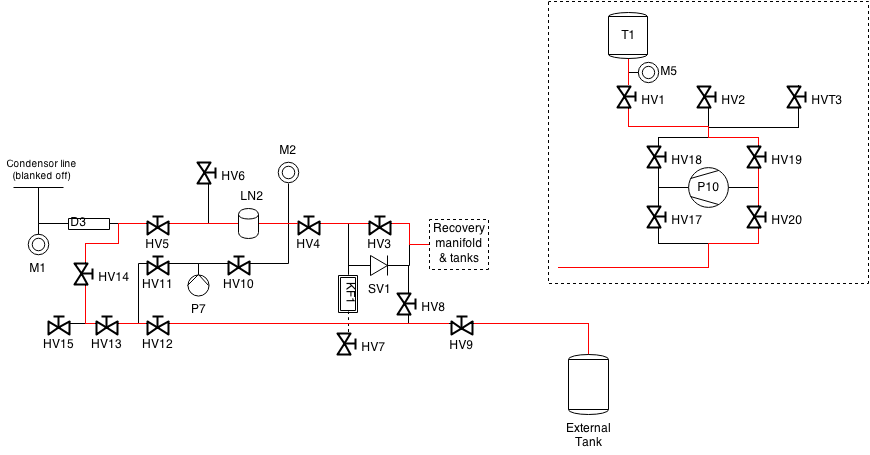
\includegraphics[width=\textwidth]{./mash-cleaning-schematic-2-gas-to-ext-tank.png}
 % he-3-transfer-04-evac-system-with-p7.png: 0x0 pixel, 0dpi, 0.00x0.00 cm, bb=
 \caption{Open valves in this order: HV1, HV19, HV20, HV3, HV4, HV5, HV14, HV13, HV12, HV9.  Wait until external tank equilibrates with T3.}
 \label{b}
\end{figure}

\begin{figure}[htbp!]
 \centering
 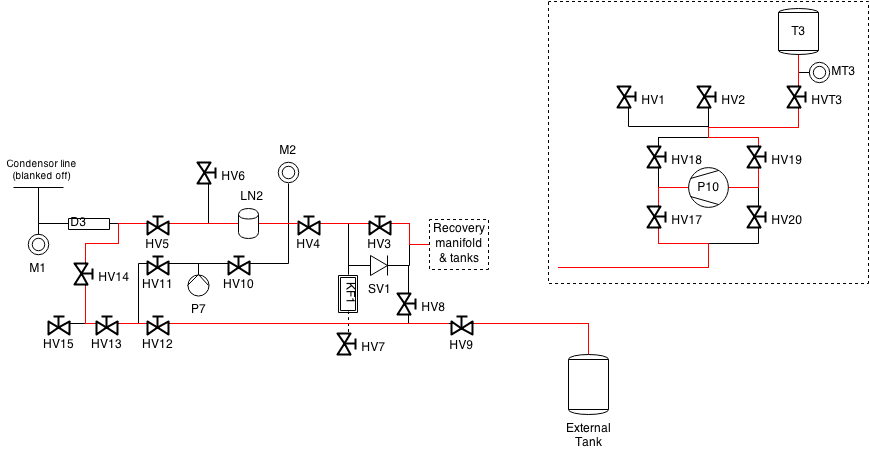
\includegraphics[width=\textwidth]{./mash-cleaning-schematic-3-pump-gas-to-ext-tank.png}
 % he-3-transfer-04-evac-system-with-p7.png: 0x0 pixel, 0dpi, 0.00x0.00 cm, bb=
 \caption{Close HV19, HV20; then open HV17 and turn on P10.  Slowly open HV19 and let M5 drop.}
 \label{c}
\end{figure}


\begin{figure}[htbp!]
 \centering
 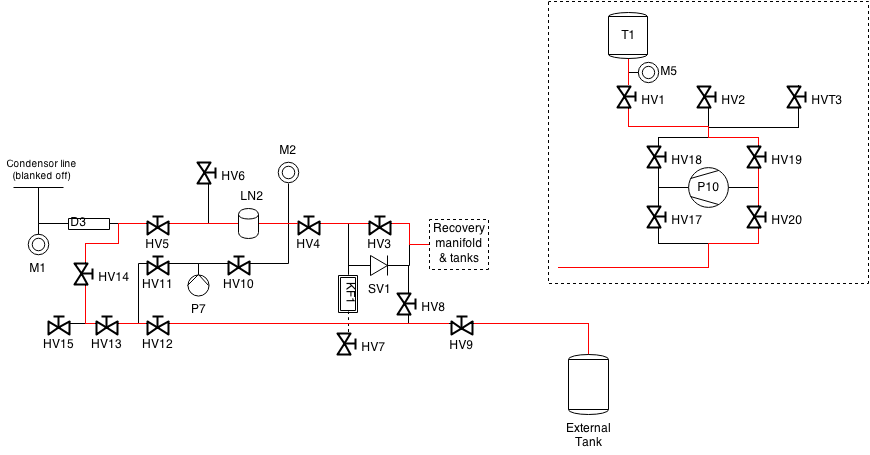
\includegraphics[width=\textwidth]{./mash-cleaning-schematic-4-gas-to-t1.png}
 % he-3-transfer-04-evac-system-with-p7.png: 0x0 pixel, 0dpi, 0.00x0.00 cm, bb=
 \caption{When M5 is around 0 mbar, close HV19, then kill P10.  Close HV17.  Open HV20 and HV19.  Wait until T1 and external tank equilibrate.}
 \label{d}
\end{figure}


\begin{figure}[htbp!]
 \centering
 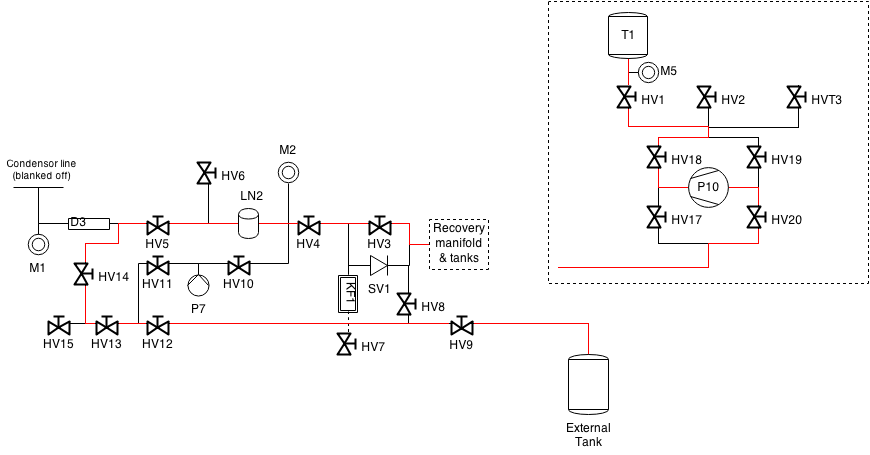
\includegraphics[width=\textwidth]{./mash-cleaning-schematic-5-pump-gas-to-t1.png}
 % he-3-transfer-04-evac-system-with-p7.png: 0x0 pixel, 0dpi, 0.00x0.00 cm, bb=
 \caption{Close HV19 and HV20.  Open HV18 and then start P10.  Slowly open HV20; wait until external tank is empty.  Close HV20, kill P10, then close HV18.}
 \label{e}
\end{figure}

\begin{figure}[htbp!]
 \centering
 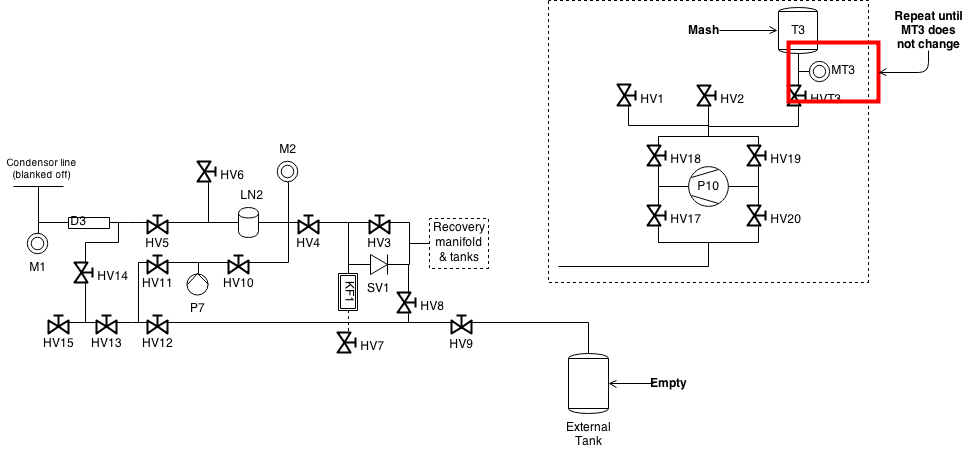
\includegraphics[width=\textwidth]{./mash-cleaning-schematic-6-repeat.png}
 % he-3-transfer-04-evac-system-with-p7.png: 0x0 pixel, 0dpi, 0.00x0.00 cm, bb=
 \caption{Repeat Steps 2-5 until M5 remains constant between passes.}
 \label{f}
\end{figure}


\begin{figure}[htbp!]
 \centering
 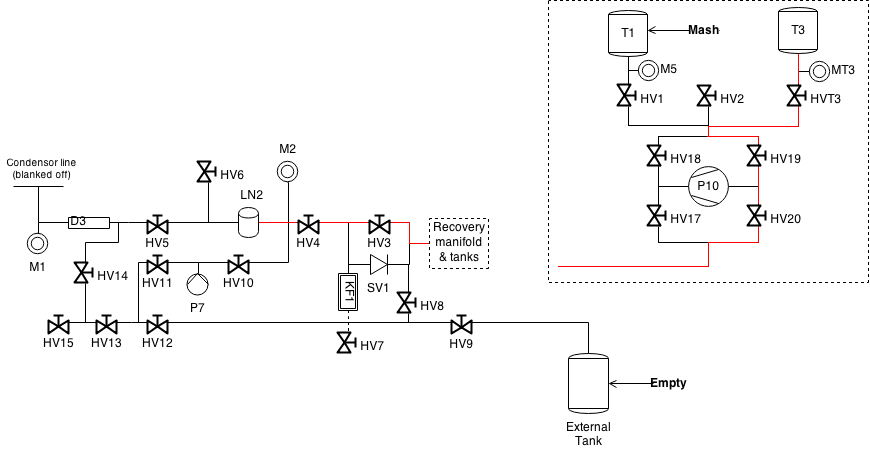
\includegraphics[width=\textwidth]{./mash-cleaning-schematic-7-measure-trapped-gas}
 % he-3-transfer-04-evac-system-with-p7.png: 0x0 pixel, 0dpi, 0.00x0.00 cm, bb=
 \caption{Close all valves, then open HV4, HV3, HV20, HV19 and HVT3.  Warm up trap and record pressure MT3 to estimate how much air was removed from mash.}
 \label{g}
\end{figure}


\end{document}
